\documentclass[10pt]{sigplanconf}

\usepackage{amsmath}
\usepackage{amsthm}
\usepackage{amssymb}
\usepackage{float}
\usepackage{pifont}
\usepackage{graphicx}
\usepackage{multirow}
\usepackage{fancyvrb}
\usepackage{url}
\usepackage{verbatim}
\usepackage{alltt}
\usepackage{semantic}
\usepackage{color}
\usepackage{setspace}
\usepackage{dblfloatfix}

\newtheorem{definition}{Definition}
\newtheorem{theorem}{Theorem}

\newcommand{\todo}[1]{\marginpar{\color{red}{\footnotesize \begin{spacing}{0.9} #1 \end{spacing}}}}

\newcommand{\sep}[0]{\; | \;}
\newcommand{\lsep}[0]{\;\; | \;\;}
\newcommand{\tsep}[0]{\; \triangledown \;}
\newcommand{\kvd}[1]{\textbf{\sffamily #1}}
\newcommand{\ident}[1]{\textnormal{\sffamily #1}}
\newcommand{\fqt}{\`{}\hspace{-0.25em}\`{}}
\newcommand{\tytag}{\overline{\tau}}
\newcommand{\tytagof}{\ident{tag}}

\newcommand{\str}[1]{\texttt{#1}}
\newcommand{\rangl}{\hspace{-0.3em}>\hspace{-0.25em}}
\newcommand{\langl}{\hspace{-0.25em}<\hspace{-0.3em}}

\begin{document}

\toappear{Unpublished draft.}
\title{Making structured data first-class citizens}

\authorinfo
  {Tomas Petricek}
  {University of Cambridge}
  {tomas.petricek@cam.ac.uk}

\authorinfo
  {Don Syme}
  {Microsoft Research, Cambridge}
  {don.syme@microsoft.com}

\maketitle

% ==================================================================================================

\begin{abstract}
% What is the problem?
% Why is it important?
% What do we do?
% What follows from that?

Accessing data in structured formats such as XML, CSV and JSON in statically typed languages 
is difficult, because the languages do not understand the structure of the data. Dynamically
typed languages make this syntactically easier, but lead to error-prone code.
Despite numerous efforts, most of the data available on the web do not come with a schema. 
The only information available to developers is a set of examples, such as typical server
responses.

We describe an inference algorithm that infers a type of structured formats including 
CSV, XML and JSON. The algorithm is based on finding a common supertype of types
representing individual samples (or values in collections).
We use the algorithm as a basis for an F\# type provider that integrates the inference
into the F\# type system. As a result, users can access CSV, XML and JSON data in a 
statically-typed fashion just by specifying a representative sample document.
\end{abstract}

% ==================================================================================================

\section{Introduction}
\label{sec:intro}

We are witnessing an explosion of digital data. International organizations \cite{data-worldbank}
and governments \cite{data-opengovuk,data-opengovusa} expose numerous datasets; 
knowledge is collected and schematized by communities \cite{data-freebase} and numerous 
commercial services provide web services for data access\footnote{As of the time of writing the 
\url{http://www.programmableweb.com} directory lists 8357 web APIs in over 60 categories.}.

Despite this fact, few strongly-typed programming languages are able to seamlessly integrate 
external information sources as if they were strongly-typed components from a programmer's 
perspective. The \emph{type provider} mechanism of F\# 3.0 \cite{providers-techreport} 
makes it possible to integrate external data sources as statically typed components
through a compiler extensibility mechanism. 

In this paper, we focus on accessing structured data formats such as CSV, XML and JSON. 
These formats are used by most of the aforementioned services. However, only a few of the
services provide a schema or other specification of the formally defines structure they use. 
Most often programmers depend on unreliable documentation and exploration of sample responses.

In this paper, we combine type inference from sample documents with F\# type provider mechanism.
The two key contributions of this paper are:

\begin{itemize}
\item We introduce F\# type providers for three most common structured document formats 
  (CSV, XML and JSON) that make structured data first-class citizens in F\# and make them
  accessible in a strongly-typed way.

\item We define types for structured data formats and present a type inference algorithm 
  based on the subtyping relation that infers type (or schema) of any structured 
  data format from a sample or a collection of samples.
\end{itemize}

We do not expect familiarity with F\# type providers, so the mechanism is introduced
along with our structural type providers in Section~\ref{sec:structural}. Type inference
is presented in Section~\ref{sec:inference}. Section~\ref{sec:operational} discusses
runtime representation of structured values and proves that it is sound with respect to
our static types. Finally, Section~\ref{sec:providers} connects the static and 
dynamic aspects by discussing how individual type providers (CSV, XML and JSON) work.

The work described in this paper is available as part of the F\# Data library, 
which is an open-source project used in practice by a number of commercial F\# users\footnote{
Available at \url{http://tpetricek.github.com/FSharp.Data}}. For this reason, we follow a 
pragmatic approach and do not ignore constraints of the real-world (such as the complexity
of the host platform or the presence of \ident{null} values).

% ==================================================================================================

\section{Structural type providers}
\label{sec:structural}

We start with a motivating example that shows how the F\# Data library simplifies working with
the JSON format and then introduce other structured type providers. At the same time, we 
introduce the F\# 3.0 type provider mechanism and highlight the key features of the type inference.

% --------------------------------------------------------------------------------------------------

\subsection{Working with JSON documents}
\label{sec:structural-json}

JSON is a popular format for data exchange on the web. It is based on data structures used in
JavaScript and uses six types (Number, String, Boolean, Array, Object and Null). Consider the
following example:
%
\begin{equation*}
\begin{array}{l}
[\; \{~\str{"name"}: \kvd{null}, \str{"age"}: 23 \}, \\
\;\;  \{~\str{"name"}: \str{"Alexander"}, \str{"age"}: 1.5 \}, \hspace{4em} \\
\;\;  \{~\str{"name"}: \str{"Tomas"} \} \; ]
\end{array}
\end{equation*}
%
In a statically typed (functional) language, JSON values would be represented using a single type. 
We could use pattern matching to check that the value matches an expected structure
and then extract the required values. Assuming \ident{data} is the above document, we print the 
names as follows:
%
\begin{equation*}
\begin{array}{l}
\kvd{match}~\ident{data}~\kvd{with}\\
|~\ident{Array items}\rightarrow\\
\quad\kvd{for}~\ident{item}~\kvd{in}~\ident{items}~\kvd{do}\\
\quad\quad\kvd{match}~\ident{item}~\kvd{with}\\
\quad\quad|~\ident{Object keys}\rightarrow\\
\quad\quad\quad\ident{printf}~\str{"\%s"}~(\ident{Map.find keys}~\str{"name"})\\
\quad\quad|~\underline{~\;}\rightarrow \ident{failwith}~\str{"Incorrect format"} \hspace{4em}\\
|~\underline{~\;}\rightarrow \ident{failwith}~\str{"Incorrect format"}
\end{array}
\end{equation*}
%
The code expects that the input is in a certain format (array of objects with the \str{"name"} field)
and it fails if the input does not match these requirements. The code is complicated for two reasons.
First, we have to repeatedly pattern match and explicitly handle failures and second, fields are
accessed indirectly (using the name as a string rather than member of a statically known type).
The first difficulty could be avoided by defining helper functions, but there is no way to avoid the 
second problem without mechanism such as type providers.

Assuming the \str{people.json} file contains the above data and \ident{data} is a string 
containing information in the same format, we can rewrite the code using \ident{JsonProvider} as 
follows (also printing the age, if it is present):
%
\begin{equation*}
\begin{array}{l}
\kvd{type}~\ident{People}~=~\ident{JsonProvider}\langl\str{"people.json"}\rangl\hspace{1em} \\[0.5em]
\kvd{let}~\ident{items}~=~\ident{People.Parse}(\ident{data})\\
\kvd{for}~\ident{item}~\kvd{in}~\ident{items}~\kvd{do}\\
\quad\ident{printf}~\str{"\%s "}~\ident{item.Name}\\
\quad\ident{Option.iter}~(\ident{printf}~\str{"(\%f)"})~\ident{item.Age}
\end{array}
\end{equation*}
%
This code achieves the same simplicity as dynamically typed programming languages, but it 
is statically type-checked.
%
\paragraph{Type providers overivew.}
The parameter \str{"people.json"} is resolved 
statically at compile-time (it has to be a constant) and is passed to the 
\ident{JsonProvider} which builds a specification of the \ident{People} type and passes it
to the F\# compiler. This type information is also available at development time allowing
advanced tooling such as code completion.

The \ident{JsonProvider} uses a type inference algorithm
(Section~\ref{sec:inference}) to infer the JSON schema from the sample file and generates
F\# types that can be used to read the data. In this case, the resulting type is a collection
of records with \ident{Name} of type \ident{string} and \ident{Age} of type \ident{decimal option}.

The type provider also specifies code that should be executed
at run-time in place of \ident{item.Name} and other operations (demonstrated in the next section).
In this example, the runtime behaviour is the same as in the version using pattern matching,
meaning that the member access throws an exception if the document does not have the expected
format. We specify this precisely in Section~\ref{sec:operational}.

\paragraph{The role of records.}
The example suggests that records play a prominent role when working with structured data. 
In fact, all three formats that we consider naturally contain a notion of record and we map 
them to F\# object types with members to support code completion.

The provider infers the types of fields (\ident{string} and \ident{decimal}) and marks the
\ident{Age} field as optional. This is not the only alternative -- we could infer a union
(sum) type consisting of two different records (with one and two fields), but that would 
complicate the processing code. In general, our inference algorithm tries to minimize the number
of unions in the inferred type.

% --------------------------------------------------------------------------------------------------

\subsection{Reading CSV files}
\label{sec:structural-csv}

The CSV format has the simplest structure of the formats that we consider. The structure is a
collection of records with fields (with names specified by the first row). When inferring the type, 
we need to infer the type of fields. Consider the following example:
%
{\small
\begin{verbatim}
  Ozone; Temp; Date
  41;    67;   2012-05-01
  36.3;  72;   2012-05-02
  12.1;  74;   3 May
\end{verbatim}
}
%
\noindent
Assuming the \str{airdata.csv} file is available locally, we can use a type provider that prints 
data obtained from a web site with live CSV data as follows:
%
\begin{equation*}
\begin{array}{l}
\kvd{type}~\ident{AirCsv}~=~\ident{CsvProvider}\langl\str{"airdata.csv"}\rangl\hspace{1em} \\[0.5em]
\kvd{let}~\ident{air}~=~\ident{AirCsv.Load}(\str{"http://data...air.csv"})\\
\kvd{for}~\ident{row}~\kvd{in}~\ident{air}~\kvd{do}\\
\quad\ident{printf}~\str{"\%s: \%d"}~\ident{row.Date row.Ozone}\\
\end{array}
\end{equation*}
%
The type of the record (\ident{row}) is inferred from the sample file, which contains three
fields. Ozone is always a numeric value, so the provider infers a \ident{decimal} type; Date uses
mixed formats, so it is inferred as \ident{string}.

\paragraph{Erasing type providers.}
At runtime, the type providers we describe use an erasure mechanism similar to Java Generics 
\cite{types-java-erasure}. When called by the compiler, a type provider also returns code that is 
executed in place of the generated types. In the above example, the compiled code looks as follows:
%
\begin{equation*}
\begin{array}{l}
\kvd{let}~\ident{air}~=~\ident{CsvFile.Load}(\str{"airdata.csv"})\\
\kvd{for}~\ident{row}~\kvd{in}~\ident{air.GetRows}()~\kvd{do}\\
\quad\ident{printf}~\str{"\%s \%f"}~\ident{row.GetString}(\str{"Date"})\\
\quad\quad\quad\quad\quad\quad\quad\;\,\ident{row.GetDecimal}(\str{"Ozone"})\\
\end{array}
\end{equation*}
%
The generated type \ident{AirCsv} is erased to an underlying type \ident{CsvFile}
that represents any CSV document. Access to a named property, such as \ident{Ozone}, is compiled into a 
method call, which reads a column using its name and converts it to a desired
type (\ident{GetDecimal}). Technical report \cite{providers-techreport} provides more details on type erasure.

% --------------------------------------------------------------------------------------------------

\subsection{Parsing RSS feeds}
\label{sec:structural-xml}

XML and JSON formats often contain collections and, especially in case of XML, the collections can
be heterogeneous containing elements of different type (i.e.~differently named XML nodes). Consider
the following RSS feed:
%
{\small{
\begin{verbatim}
  <rss version="2.0"><channel>
    <title> BBC News - Europe </title>
    <item><title> Kurdish activists 
        killed in Paris </title></item>
    <item><title> German MPs warn 
        over UK EU exit </title></item>
  </channel></rss>
\end{verbatim}
}}
%
\noindent
The \ident{channel} node contains a single \ident{title} node and multiple \ident{item} nodes.
Moreover, \ident{title} nodes always contain only a single child, which is a plain text.

When extracting data from similar XML documents, we often need to get nodes of a specific name
or get the content of a node. The type provider we present is optimized for this style of access
and allows processing the feed as follows:
%
\begin{equation*}
\begin{array}{l}
\kvd{type}~\ident{RssFeed}~=~\ident{XmlProvider}\langl\str{"rss.xml"}\rangl\hspace{1em} \\[0.5em]
\kvd{let}~\ident{rss}~=~\ident{RssFeed.Load}(\str{"http://bbc.co.uk/..."})\\
\ident{printf}~\str{"\%s "}~\ident{rss.Title}\\
\kvd{for}~\ident{item}~\kvd{in}~\ident{rss.GetItems}()~\kvd{do}\\
\quad\ident{printf}~\str{"\%s "}~\ident{item.Title}\\
\end{array}
\end{equation*}
%
In this example a heterogeneous collection (\ident{rss}) is represented as a type that contains
a member (\ident{Title}) for an element that is present exactly once and a method 
(\ident{GetItems}) for elements that are present multiple times. As a further simplification,
if an element contains only a primitive value (such as \ident{Title}) it is represented as a 
value of primitive type.

\paragraph{Collections and union types.}
As an alternative, the inference could produce a collection of sum type (with a case for \ident{item}
and a case for \ident{title}). This alternative is useful for documents with complicated structure 
(such as XHTML files), but less useful for files with simpler structure such as web server responses,
data stores and configuration files. 

Moreover, our approach has a nice property that the following two, semantically equivalent, XML 
nodes are exposed a type with the same public interface:
%
{\small{
\begin{verbatim}
<author name="Tomas" age="27" />
<author><name>Tomas</name><age>27</age></author>
\end{verbatim}
}}
%
\noindent
In both cases, the type is a record with two properties, typed \ident{string} and \ident{int} 
respectively. The discussion in Section~\ref{sec:inference} uses the simple model (using sum types)
and the inference described in the above examples is discussed in Section~\ref{sec:more-collections}.

% ==================================================================================================

\section{Structural type inference}
\label{sec:inference}

The type inference algorithm for structured data is based on a subtyping relation. When inferring 
the type of a specified document, we infer (the most specific) types of individual values, such as
CSV rows or JSON nodes, and then find the common supertype of values in a given dataset.

We define \emph{structural type} $\tau$ which is a type of the structured data. Note that this type
is distinct from the F\# types (type provider maps \emph{structural types} to ordinary F\# types). 
The subtyping relation is not mapped to a subtyping relation between F\# types, but it holds at 
runtime (meaning that an operation on a super-type is allowed on all subtypes). The operational 
aspects are discussed in Section~\ref{sec:operational}.

% --------------------------------------------------------------------------------------------------

\subsection{Structural types}
\label{sec:inference-types}

The grammar below defines \emph{structural type} $\tau$. Records and record fields are named with
names $\nu$. Record fields are marked with a qualifier $\delta$ which is either $?$ for optional
fields or empty for required fields.
%
\begin{equation*}
\begin{array}{rl}
\multicolumn{2}{l}{
  \tau \; ::= \, \top \lsep \kvd{null}
}\\  
\;\;  &\lsep \tau + \ldots + \tau \lsep [\tau]\\
      &\lsep \nu_{\ident{opt}} \; \{ \delta_1 \nu_1 : \tau_1, \; \ldots \; , \delta_n \nu_n : \tau_n \} \\
      &\lsep \ident{int} \lsep \ident{decimal} \lsep \ident{float} \lsep \ident{bool} \lsep \ident{string} \\
\end{array}
\end{equation*}
%
In structured documents such as CSV, XML and JSON, the record type is the most prominent. We use 
it to type rows of a CSV file, the type of XML nodes and JSON objects.

To support these scenarios, records may be optionally named with $\nu_{\ident{opt}}$. For example,
records representing XML nodes are named with the name of the node. Fields of a record
are named with names $\nu_1, \ldots, \nu_n$ and each field may be marked as optional (we write 
$\ident{?foo}$ for an optional field and $\ident{foo}$ for a mandatory field).

We start by using a simple collection type $[\tau]$ together with a union type $\tau + \ldots + \tau$.
As discussed earlier, the library implements a more sophisticated type inference for heterogeneous
collections, which is discussed in Section~\ref{sec:more-collections}. Aside from collections, a 
union type appears when the user provides multiple samples with different structure.

\paragraph{Alternative representations.}
The record type in our definition is more complex than in other systems, so it is worth discussing 
the alternatives and justifying our design.\todo{Ref. some ``other system'' here?}

Firstly, we could use an optional type to represent optional fields. However, none of the structured
formats we consider (CSV, XML, JSON) uses optional types elsewhere, so we could represent types that
are not inhabited in any our use case. Secondly, we could replace named fields and (optionally) named
records with a type assigning a name to any other type (such as $\tau~\kvd{as}~\nu$). Again, our use
cases only name record types and their fields, so types such as $[\ident{int}]~\kvd{as}~\nu$ would not
be inhabited.

Finally, one of the crucial operations in the system is finding common types for multiple record values.
For example, for values $\{ \ident{a} = 5 \}$ and $\{ \ident{a} = 10, \ident{b} = \kvd{true} \}$
we want to obtain a type $\{ \ident{a} : \ident{int}, \ident{?b} : \ident{bool} \}$. This would require
complex rules matching records of named optional types (and records of optional named types).

\begin{figure}
\begin{center}
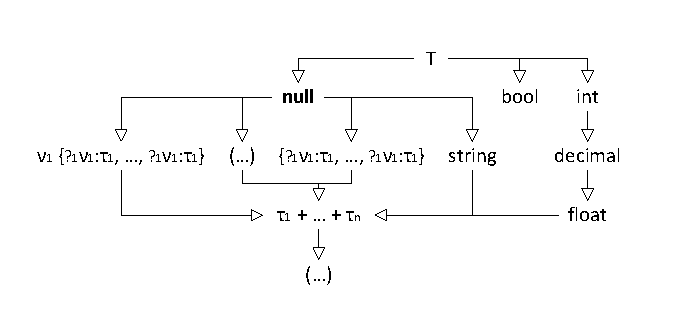
\includegraphics[scale=0.85,trim=10mm 4mm 12mm 9mm,clip]{images/hierarchy.pdf} % left bottom right top
\end{center}
\vspace{-1em}
\caption{Subtype relation between structural types}
\label{fig:subtyping-diagram}
\end{figure}

% --------------------------------------------------------------------------------------------------

\subsection{Subtyping relation}
\label{sec:inference-subtyping}

To provide a basic intuition, the subtyping relation between structured types is
informally demonstrated in Figure~\ref{fig:subtyping-diagram}. The formal definition
looks as follows:

\begin{definition}
A subtyping relation between structural types (we write $\tau_1 :> \tau_2$ to denote
that $\tau_2$ is a subtype of $\tau_1$) is defined as (a transitive reflexive closure of):
%
\begin{align}
\label{eq:sub-num}
\ident{float}~:>~\ident{decimal}~&:>~\ident{int}\\
\label{eq:sub-null}
\tau :> \kvd{null} \quad (\textnormal{iff}~\tau \notin &\{\top, \ident{bool}, \ident{int}, \ident{decimal}, \ident{float} \})\\
\label{eq:sub-top}
\tau :> \top \quad &(\textnormal{for all}~\tau)\\
\label{eq:sub-col}
[\tau_1] :> [\tau_2] \quad &(\textnormal{if}~\tau_1 :> \tau_2)\\
\label{eq:sub-union1}
\tau_1 + \ldots + \tau_n :> \tau \quad &(\textnormal{if}~\exists i . \tau_i :> \tau)
\end{align}
\vspace{-1.5em}
\begin{equation}
\label{eq:sub-union2}
\begin{array}{l}
\tau_1 + \ldots + \tau_n :> \tau_1' + \ldots + \tau_m' \quad \\[0.2em]
\quad\quad (\textnormal{if}~\forall i \in 1 .. m. \;\exists j \in 1 .. n~\textnormal{such}~\textnormal{that}~\tau_j :> \tau_i')
\end{array}
\end{equation}
\vspace{-0.4em}
\begin{equation}
\label{eq:sub-record}
\begin{array}{l}
\nu_{\ident{opt}} \; \{ \delta_1 \nu_1 : \tau_1, \; \ldots \; , \delta_n \nu_n : \tau_n \} :>\\
\nu_{\ident{opt}}' \; \{ \delta_1' \nu_1' : \tau_1', \; \ldots \; , \delta_m' \nu_m' : \tau_m'\\[0.3em]
\;\;(\textnormal{\small if $\exists$ injective}~p : \{1 .. m\} \rightarrow \{1 .. n\}~\textnormal{\small such that}\\
\quad\forall i \in 1 .. n. (i \notin p[\{1 .. m\}] \implies \delta_i = ?)~\textnormal{\small and}\\
\quad\forall i \in 1 .. m. (\tau_{p(i)} :> \tau_i' \wedge \delta_i' = ? \implies \delta_{p(i)} = ? ) )
\end{array}
\end{equation}
\end{definition}
%
\noindent
Here is a summary of the key aspects of the definition:

% --------------------------------------------------------------------------------------------------

\begin{figure*}[t]
\vspace{-2em}
\small{
Assume that the record fields are ordered to make $k$ the largest index such that
it holds that $\nu_i = \nu'_i \Leftrightarrow i \leq k$.
}
\begin{equation*}
\inference[(record)\;]
  { \tau_i \tsep \tau'_i \vdash  \tau''_i \quad (\forall i \in 1 .. k) \quad\quad
    \textnormal{let}~\delta''_i = ?~$ iff $~\delta_i = ? ~\vee~ \delta'_i = ? }
  { \begin{array}{c}
    \nu_{\ident{opt}} \; \{ \delta_1 \nu_1 : \tau_1, \; \ldots \; , \delta_n \nu_n : \tau_n \} \tsep
    \nu_{\ident{opt}} \; \{ \delta'_1 \nu'_1 : \tau'_1, \; \ldots \; , \delta'_m \nu'_m : \tau'_m \} \vdash\\
    \nu_{\ident{opt}} \; \{ \delta''_1 \nu_1 : \tau''_1, \; \ldots \; , \delta''_n \nu_k : \tau''_k,
                            ?\nu_{k+1} : \tau_{k+1}, \ldots, ?\nu_n : \tau_n,
                            ?\nu'_{k+1} : \tau'_{k+1}, \ldots, ?\nu'_m : \tau'_m \}
    \end{array} }
\end{equation*}
\vspace{0.5em}

\small{
Assume that the union cases are ordered to make $k$ the largest index such that it holds that 
$\tytagof(\tau_i) = \tytagof(\tau'_i) \Leftrightarrow i \leq k$\newline
and assume that $m', n'$ are indices such that it holds that $\tau_i = \kvd{null} \Leftrightarrow i > n'$ and
$\tau_i' = \kvd{null} \Leftrightarrow i > m'$.
}
\begin{equation*}
\inference[(union-1a)\;]
  { \tau_i \tsep \tau'_i \vdash  \tau''_i \quad (\forall i \in 1 .. k) &
    \exists i. (\tau_i = \kvd{null} \vee \tau_i' = \kvd{null}) &
    \nexists i. (\kvd{null} :> \tau_i \vee \kvd{null} :> \tau_i') }
  { (\tau_1 + \ldots + \tau_n) \tsep (\tau'_1 + \ldots + \tau'_m) \vdash
    (\tau''_1 + \ldots + \tau''_k +
    \tau_{k+1} + \ldots \tau_{n'} + \tau'_{k+1} + \ldots + \tau'_{m'} + \kvd{null}) }
\end{equation*}
\begin{equation*}
\inference[(union-1b)\;]
  { \tau_i \tsep \tau'_i \vdash  \tau''_i \quad (\forall i \in 1 .. k) &
  	\textnormal{\footnotesize Premise of (union-1a) does not hold} }
  { (\tau_1 + \ldots + \tau_n) \tsep (\tau'_1 + \ldots + \tau'_m) \vdash
    (\tau''_1 + \ldots + \tau''_k +
    \tau_{k+1} + \ldots \tau_{n'} + \tau'_{k+1} + \ldots + \tau'_{m'}) }
\end{equation*}
\vspace{0.5em}

\small{
The remaining cases do not have any assumptions:}

\begin{equation*}
\textnormal{\footnotesize{(union-2)}}\;\;
\inference
  {\exists i . \tytagof(\tau_i) = \tytagof(\tau) & \tau \tsep \tau_i \vdash \tau_i'}
  {\tau \tsep (\tau_1 + \ldots + \tau_n) \vdash (\tau_1 + \ldots + \tau_i' + \ldots + \tau_n)}
\quad\quad
\inference
  {\nexists i . \tytagof(\tau_i) = \tytagof(\tau)}
  {\tau \tsep (\tau_1 + \ldots + \tau_n) \vdash (\tau_1 + \ldots + \tau_n + \tau)}
\end{equation*}


\begin{equation*}
\inference[(list)\;]
  {\tau \tsep \tau' \vdash \tau''}
  {[\tau] \tsep [\tau'] \vdash [\tau'']}
%
\quad\quad\quad
%
\inference[(num)\;]
  {\tau :> \tau'}
  {\tau \tsep \tau' \vdash \tau}\;
\inference
  {\tau :> \tau'}
  {\tau' \tsep \tau \vdash \tau_1}
\;(\tau, \tau' \in \{\ident{int}, \ident{decimal}, \ident{float} \})
\end{equation*}

\begin{equation*}
\textnormal{\footnotesize{(top)}}\;\;
\top \tsep \tau \vdash \tau \quad
\tau \tsep \top \vdash \tau
%
\quad\quad\quad
%
\textnormal{\footnotesize{(equal)}}\;\;
\tau \tsep \tau \vdash \tau
%
\quad\quad\quad
%
\inference[(null)\;]
  {\tau :> \kvd{null}}
  {\tau \tsep \kvd{null} \vdash \tau}\;
\inference
  {\tau :> \kvd{null}}
  {\kvd{null} \tsep \tau \vdash \tau_1}
\end{equation*}

\vspace{0.5em}
\small{
If no other inference rules applies, then the following rule is used:}
\begin{equation*}
\textnormal{\footnotesize{(union-3)}}\;\;
\tau_1 \tsep \tau_2 \vdash \tau_1 + \tau_2
\end{equation*}
\vspace{-1em}
\caption{Inference judgements that define the common supertype relation}
\label{fig:subtyping-cst}
\end{figure*}

% --------------------------------------------------------------------------------------------------

\begin{itemize}
\item Numeric types correspond to F\# types. We aim to infer a single most precise numeric type that 
  can represent all values from a sample dataset. We order types by the ranges they represent (\ref{eq:sub-num});
  \ident{int} is 32-bit integer, \ident{decimal} has higher precision than \ident{float},
  but smaller range. 

\item The \kvd{null} value is a valid value of all record and union types as well as \ident{string}, but
  it is not a valid value of other primitive types, also called \emph{value types} (\ref{eq:sub-null}).

\item There is a top type (\ref{eq:sub-top}), but no bottom type. However it is possible to find common 
  supertype of any two types, because a union type $\tau_1 + \ldots + \tau_n$ is a supertype of all its 
  components (\ref{eq:sub-union1}).

\item However, given two types, there may be multiple common supertypes that are not related by
  subtyping. For example, arising from rules (\ref{eq:sub-union1}) and (\ref{eq:sub-record}). 

\item A record type is a supertype of another record type if it contains all its fields (optional fields
  have to remain optional) and all other fields are optional. Records are only related if they are both 
  anonymous or if they have the same name (\ref{eq:sub-record}).
\end{itemize}

\noindent
Some of the aspects (such as \kvd{null} type and primitive numeric types) may appear overly complicated
and F\# specific. This paper aims to describe a realistic system rather than an (overly) simplified 
model. 

Analogous problems will appear with most real-world languages (JVM languages have both \kvd{null}
and multiple numeric types; OCaml has multiple numeric types and would have to represent \kvd{null} with 
an explicit option type).

% --------------------------------------------------------------------------------------------------

\subsection{Common supertype relation}
\label{sec:inference-commonsuper}

As mentioned earlier, the structured type inference relies on a finding common supertype. However,
the partially ordered set of types does not have a unique greatest lower bound. For example, record types
$\{\ident{a}:\ident{int}\}$ and $\{\ident{b}:\ident{bool}\}$ have common supertypes
$\{\ident{?a}:\ident{int}, \ident{?b}:\ident{bool}\}$ and $\{\ident{a}:\ident{int}\} + \{\ident{b}:\ident{bool}\}$
which are unrelated.
Our inference algorithm aims to infer records when possible (the first case). To do that, we use
a \emph{common supertype} relation: 

\begin{definition}
A \emph{common supertype} of types $\tau_1$ and $\tau_2$ is a type $\tau$ (written $\tau_1 \triangledown \tau_2 \vdash \tau$)
obtained according to the inference rules in Figure~\ref{fig:subtyping-cst}.
\end{definition}

Notable aspects of the definition including the $\tytagof$ function are discussed below.
The common supertype relation finds a single supertype (among several possibilities). 
The following theorem states that the found type is, indeed, a common supertype:

\begin{theorem}
If $\tau_1 \triangledown \tau_2 \vdash \tau$ then $\tau :> \tau_1$ and $\tau :> \tau_2$.
\end{theorem}
\begin{proof}
By analysis of the inference rules in Figure~\ref{fig:subtyping-cst}.
\end{proof}

\noindent
When finding a common supertype of two records (record), we return a record type that has the union
of fields of the two arguments. The types of shared fields are common supertypes of their respective
types. Fields that are present in only one record or are optional in one of the records are marked
as optional in the result.

Finding a common supertype of union types (union-1) is more complicated. Our definition aims to add
as few additional cases as possible, without creating nested union types (e.g. $\ident{int} + (\ident{bool} + \ident{decimal})$).
This is done by grouping types that have a common supertype which is not a union type (in the previous
example \ident{int} with \ident{decimal} and \ident{bool}). We then find common supertype of each group and create union
of these types (in our example $\ident{decimal} + \ident{bool}$).

The types are grouped by a \emph{tag} that determines the kind of type (number, record, etc.)
and is defined as:
%
\begin{equation*}
\begin{array}{rl}
\multicolumn{2}{l}{
\tytag \; ::= \; \ident{string} \lsep \ident{bool} \lsep \ident{number} 
}\\  
\;\;  &\lsep \ident{record} \lsep \ident{named}~\nu \lsep \ident{union} \lsep \ident{list}
\end{array}
\end{equation*}
%
The tag of a type is obtained using a function $\tytagof$. It holds that two types with the 
same tag (which are not unions) have a common supertype that is also not a union:
%
\begin{equation*}
\begin{array}{ll}
\tytagof : \tau \rightarrow \tytag\\
\tytagof(\ident{string}) &= \ident{string}\\
\tytagof(\ident{bool}) &= \ident{bool}\\
\tytagof([\tau]) &= \ident{list}\\
\tytagof(\tau + \ldots + \tau) &= \ident{union}\\
\tytagof(\ident{int}) = \tytagof(\ident{decimal}) = \tytagof(\ident{float}) &= \ident{number}\\
\tytagof(\{ ?_1 \nu_1 : \tau_1, \; \ldots \; , ?_n \nu_n : \tau_n \}) &= \ident{record}\\
\tytagof(\nu\; \{ ?_1 \nu_1 : \tau_1, \; \ldots \; , ?_n \nu_n : \tau_n \}) &= \ident{named}~\nu
\end{array}
\end{equation*}
%
The function is undefined for the $\top$ and $\kvd{null}$ types, but this is not a 
problem because these types are never used as arguments in Figure~\ref{fig:subtyping-cst}.
Assuming that no primitive value has a type $\top$, the top type is always eliminated in the
(top) rule and so it cannot appear as a member of union in any of the (union) rules.

The \kvd{null} type is handled explicitly. When combining two unions, we only include 
\kvd{null} type explicitly if it is present in one of the original unions and none of the 
other types permit \kvd{null} as a valid value (union-1a), otherwise \kvd{null} is excluded.

\paragraph{Minimising unions.}
We stated earlier that the common supertype relation minimises the use of union types 
(by preferring common numeric types or common record types when possible). This property
can be stated and proved formally:
%
\begin{theorem}
If $\tau :> \tau_1$ and $\tau :> \tau_2$ and $\tau$ is not a union type and
$\tau_1 \tsep \tau_2 \vdash \tau'$ then $\tau'$ is not a union type.
\end{theorem}
\begin{proof}
The only rule that introduces an union type is (union-3). By examining possible structures
of $\tau$, we see that the rule can only be used if there is no other supertype of 
both $\tau_1$ and $\tau_2$.
\end{proof}

% ==================================================================================================

\begin{figure*}[t]
\begin{equation*}
\begin{array}{l}
\kvd{let}~\ident{GetFloat value} =\\
\quad\kvd{match}~\ident{value.GetNumber}()~\kvd{with}\\
\quad|~\ident{Choice1 n} \rightarrow \ident{floatOfInt n}\\
\quad|~\ident{Choice2 d} \rightarrow \ident{floatOfDecimal d}\\
\quad|~\ident{Choice3 f} \rightarrow \ident{f}\\
\end{array}
\quad\quad
\begin{array}{l}
\kvd{let}~\ident{GetDecimal value} =\\
\quad\kvd{match}~\ident{value.GetNumber}()~\kvd{with}\\
\quad|~\ident{Choice1 n} \rightarrow \ident{decimalOfInt n}\\
\quad|~\ident{Choice2 d} \rightarrow \ident{d}\\
\quad|~\underline{~\;} \rightarrow \bot\\
\end{array}
\quad\quad
\begin{array}{l}
\kvd{let}~\ident{GetInt value} =\\
\quad\kvd{match}~\ident{value.GetNumber}()~\kvd{with}\\
\quad|~\ident{Choice1 n} \rightarrow \ident{n}\\
\quad|~\underline{~\;} \rightarrow \bot
\end{array}
\end{equation*}

\caption{Auxiliary functions for accessing numeric values}
\label{fig:runtime-functions}
\end{figure*}

\begin{figure*}[!b]
\hrulefill

\begin{equation*}
\inference
  {\ident{GetInt}(\rho)\downarrow}
  {\rho \in \ident{int}}
\quad
\inference
  {\ident{GetDecimal}(\rho)\downarrow}
  {\rho \in \ident{decimal}}
\quad
\inference
  {\ident{GetFloat}(\rho)\downarrow}
  {\rho \in \ident{float}}
\quad
\inference
  {\ident{GetBool}(\rho)\downarrow}
  {\rho \in \ident{bool}}
\quad
\inference
  {\ident{IsNull}(\rho)=\kvd{true}}
  {\rho \in \kvd{null}}
\end{equation*}\vspace{0.4em}
\begin{equation*}
\inference
  {\rho \in \kvd{null} \vee \ident{GetString}(\rho)\downarrow}
  {\rho \in \ident{string}}
\quad
\inference
  {
  \rho \in \kvd{null} \vee (\ident{GetItems}(\rho)\downarrow \wedge
  \forall \rho' \in \ident{GetItems}(\rho). \rho' \in \tau)
  }
  {\rho \in [\tau]}
\quad
\inference
  { \rho \in \kvd{null} ~\vee \exists i. \rho \in \tau_i }
  { \rho \in \tau_1 + \ldots  + \tau_n }
\end{equation*}\vspace{0.4em}
\begin{equation*}
\inference
  {
  \rho \in \kvd{null} \vee \forall i\in 1 .. n.
  \big((\ident{GetField}(\rho, \nu_{\ident{opt}}, \nu_i) = \ident{Some}(\rho') ~\wedge~ \rho' \in \tau_i) \vee 
  (\ident{GetField}(\rho, \nu_{\ident{opt}}, \nu_i) = \ident{None} ~\wedge~ \delta_i =~ ?)\big)
  }
  {\rho \in \nu_{\ident{opt}} \; \{ \delta_1 \nu_1 : \tau_1, \; \ldots \; , \delta_n \nu_n : \tau_n \}}
\end{equation*}

\caption{Inference rules that define type of a runtime value}
\label{fig:runtime-type}
\end{figure*}
\section{Runtime representation}
\label{sec:operational}

In the previous section, we defined static type of structured documents and we defined the 
subtyping relation between types. In this section, we add the operational semantics -- we 
describe runtime representation of values and discuss when a value belongs to a type. This also
clarifies what structural changes in the input document do not break programs written using 
inferred types.

As discussed earlier, the structured type providers discussed in this article use the 
\emph{type erasure} mechanism. At runtime, all values are represented using a single type that
provides a number of operations that view the value as a value with a certain structure.
If a value does not match the required structure, the operation is undefined.

The key claim that we make in this (and the next) section is that, if we have an (inferred) type $\tau_1$ and
a value that does not contain \kvd{null} and belongs to a type $\tau_2$ which is a subtype 
of $\tau_1$ ($\tau_2 :> \tau_1$), then all operations that may be called by user code to 
access the value are defined.

At runtime, a value from a structured document is represented using a single type that
we call \ident{Value}\footnote{Here we slightly diverge from the actual representation in 
the F\# Data library, which uses a different representation for every format, although they 
mostly share the structure discussed here.}. The type is a record of functions that can be 
called to obtain a value with a specified format (and may be undefined if the required format
is not available):
%
\begin{equation*}
\begin{array}{lcl}
\ident{GetBool} &:& \ident{Value} \rightarrow \ident{bool} \\
\ident{GetNumber} &:& \ident{Value} \rightarrow \ident{int}+\ident{decimal}+\ident{float} \\
\ident{GetString} &:& \ident{Value} \rightarrow \ident{string} \\
\ident{IsNull} &:& \ident{Value} \rightarrow \ident{bool}\\
\ident{GetItems} &:& \ident{Value} \rightarrow \ident{Value list}\;\\
\ident{GetField} &:& \ident{Value} \times \ident{string option} \times \ident{string} \\
                  && \quad \rightarrow \ident{Value option}
\end{array}
\end{equation*}
%
The first three operations extract a primitive value. Note that \ident{GetNumber} may return
any of the supported numeric types. The F\# runtime provides a conversion from \ident{int}
to \ident{decimal} and from \ident{decimal} to \ident{float}. These are used in Figure~\ref{fig:runtime-functions}
to define functions that get a value of a specific numeric type and convert values. The conversion
may lose precision, but it does not overflow.

The \ident{GetField} operation returns the value of a field -- it takes \ident{string option} 
which is the name of the desired record type (or \ident{None} if the record is anonymous) and
the name of the field. The operation returns \ident{None} if the value is a record with matching
name, but the field is missing. 

\paragraph{Type of values.} Next, we define what does it mean for a runtime \ident{Value} to 
have a type $\tau$ and show that a value of a certain type is also a value of all its supertypes.

\begin{definition}
Given a \ident{Value}~$\rho$, the value belongs to a type $\tau$ (written
$\rho \in \tau$) as defined by inference rules in Figure~\ref{fig:runtime-type}
(we write $f(x)\downarrow$ to mean that $f(x)$ is defined).
\end{definition}

\noindent
The definition matches the intuitive understanding presented so far. For numeric types, a value is 
of a specific type (e.g.~\ident{decimal}) if \ident{GetNumber} returns the exact type or a type that
can be converted to it (e.g.~from \ident{int}). When \ident{IsNull} is true, the value belongs to 
any record and union type, as well as to the \ident{string} type.

A value is of a union type if it belongs to any of the types that form the union. In order to belong
to a specific record type, the \ident{GetField} function needs to be defined for all fields and it
has to return \ident{Some} for all required fields. Finally, no value belongs to the $\top$ type.

\paragraph{Flexibility.} When inferring document type from a sample, we can expect that future
inputs will not have exactly the same structure (for example, a web service may add additional 
field in the result). 


~
\begin{itemize}
\item Using smaller number is allowed (but not bigger)
\item Using null in place of string/record/union
\item Using subtypes as elements of a collection
\item Adding fields is fine (or, in fact, having records that contain fields 
  associated with multiple different record names)
\end{itemize}

~

~

~

\paragraph{Soundness of subtyping.}
The type inference algorithm proceeds by finding a common supertype of sample values. In order for
this to be valid, a runtime value that has a type $\tau$ also needs to belong to all supertypes of
$\tau$. This is proved by the following theorem:

\begin{theorem}
Assuming $\tau_1 :> \tau_2$ and a value $\rho$ has a type $\tau_2$ 
(written $\rho \in \tau_2$) then the value $\rho$ has a type $\tau_1$
($\rho \in \tau_1$).
\end{theorem}
\begin{proof}
By analysis of the cases in the subtyping relation as defined in Section~\ref{sec:inference-subtyping}.
Assuming runtime requirements hold for $\tau_2$, the runtime requirements for $\tau_1$ hold as well.
\end{proof}

% ==================================================================================================

\section{Individual providers}
\label{sec:providers}

now we have type inference and runtime representation, so we can connect the two (somehow..)

\subsection{CSV files}
Given a CSV file

\begin{theorem}
Given a CSV file with inferred type $\tau$, and a value $\rho$ that belongs to this type,
all accessors in the code written by the user are always defined.
\end{theorem}

\subsection{JSON documents}

\section{Additional stuff}

\subsection{Collections}
\label{sec:more-collections}

\subsection{Units of measure}
\label{sec:more-units}



\newpage
~
\newpage










































\bibliographystyle{abbrvnat}
\bibliography{structural}

\end{document}
